\documentclass[10pt,twocolumn]{jsarticle}
  \usepackage{graphicx}
  \usepackage[dvipdfmx]{color}
  \usepackage{url}
  \usepackage [top=20mm, bottom=20mm, left=20mm, right=20mm] {geometry}


\begin{document}

\section{はじめに}


えっと,スマホアプリをpythonで書くことはすごくめんどくさ(一般的ではな)くて,
基本的にスマホアプリは,androidならjavaという言語を使ってandroid studioというツールで,iphoneならswiftという言語を使ってXcodeというツールで作成します(iphone版とandroid版があるのはそういうことです).pythonはGUIが弱い(画面表示が苦手)ので,そもそもアプリに向いていません(主観).

それで,一口にプログラミングといってもだいたい下の三種類くらいに分類されて,それぞれ適切な言語がだいぶ違います(主観).

\begin{itemize}
  \item 1.目に見えるもの(スマホアプリとか)
  \item 2.自動化系(めんどくさい処理を自動化)
  \item 3.変態(プログラミング言語を作るやつら)
\end{itemize}



この中で,いわゆる計算機科学的視点から見ると,
1はあまり良くありません(いいプログラミング習慣がつきにくい(これはやっていくとわかると思います)).

\section{どれからやるべきか}
ぼくは自動化方面(数値計算とかそっちあたり)から入門したのでなんとも言えませんが,
スマホアプリを作りたいってことは1番目を目指していると思います.スマホのようにプラットフォームに依存しない一番目として,webページを作ってみるのがいいんじゃないでしょうか.
単純なwebページにはプログラミングも何もないですが,ある程度凝ったものになると程よくプログラミング習慣をつけれると思います.
一応アプリ開発を最初からゴリゴリやることはできますが,プログラミングに存在している概念(スコープとかその辺)さえつかめば,複数のプログラミング言語を用いて開発ができるので(もちろん,プログラミング言語によって異なる"単語"は覚えなくてはいけませんが),比較的優しいプログラミング言語から始めることをお勧めします.気持ちとしては,日本語と韓国語は表記が全く異なるけれど,文法上のルールはほとんど同じなので,単語さえggれば十分に読み書きできる.といったところでしょうか(わかりにくかったらごめん)

\section{どんな言語がいいのか}
プログラミング言語といっても星の数ほどありますよね.どれを選んだらいいかわかりにくいと思います.分類にもよりますが,基本的にプログラミング言語は静的型付けと動的型付けに分類できて,
pythonは前者,c,c++は後者に当たります.数学的な厳密さを求めるなら後者なのですが,如何せん学習が難しいので最初は前者をお勧めします.

また,pythonやprocessing以外をwindowsで開発することは個人的には苦行でしかないです(設定が本当にめんどくさくてハゲそうになります).なのでvirtualboxのような仮想化システムを使ってwindows上でubuntuなどのlinuxを使って開発することをお勧めします.

\section{環境の作り方}
プログラミングをする環境の作り方(コンパイラーやエディターの設定等)ですが,基本的には参考とする文献やwebページに書いてあると思います.
先ほど,processingとpythonはwindowsで開発できることをにおわせる記述をしましたが,まさにその通りです.
processingはこいつをダウンロードすれば基本なんでもできます.\url{https://processing.org/download/}

pythonはこいつをダウンロードすれば問題ありません.\url{https://www.anaconda.com/products/individual}

これ以外はめんどくさすぎてwindowsで触ったことがありません.なので環境の作り方とか知らないごめん.

\section{学習の仕方}
プログラミングの概念であったり手続きを学習したいのならただひたすら書きます.そして人が書いたコードを読みます(競技プログラミングにおいてはこれが重要です),そうでなければ延々とコマンドを紙に書いて暗記できるようにしましょう(情報のテストは本当にクソです.手書きさせんな).英単語とは異なり,プログラミングをする環境にはネットがあります.なのでわからなくなったらすぐにggります.写経もかまいませんが,写経しているコードがどのような動作をするか理解した上で写経しないとあまり意味はありません.とりあえずgithubに登録しましょう(n予備校にやり方は全部書いてあります).言ってくれればぼくの書いているコードをわたしますし,コードレビューもします.

\section{各分野の特色と参考になるもの}
それでは,一つづつ挙げていきます.

\subsection{0について}
何も作らずにやり方のみを学習する場合.

\begin{itemize}
  \item pythonについて:SFCの人が書いてるっぽい \url{https://github.com/kaityo256/python_zero}

  \item pythonについて:segaが書いてくれてるぜ \url{http://techblog.sega.jp/entry/2020/04/27/100000}

  \item c++について:ドワンゴの中の人が書いてるっぽい \url{https://github.com/EzoeRyou/cpp-intro}

  \item c++について:今日プロの人が書いてるよ \url{https://atcoder.jp/contests/APG4b}

\end{itemize}


\subsection{1について}
スマホアプリは大変なので,webページを作ることやそれ以外の優しい言語を用いて表現する系統をお勧めします.
そんな時に便利なのが,N予備校のプログラミング入門webアプリです.これの1章2章を読むとwebページを作れるようになります.

\url{https://www.nnn.ed.nico/}

\hrulefill

これでもいいんですが,なんか面白くないし物足りないなぁと思ったら,こういう画像を作るのはどうでしょうか?
\begin{figure}[h]
  \begin{tabular}{c}
  \begin{minipage}[t]{1\hsize}
  \begin{center}
  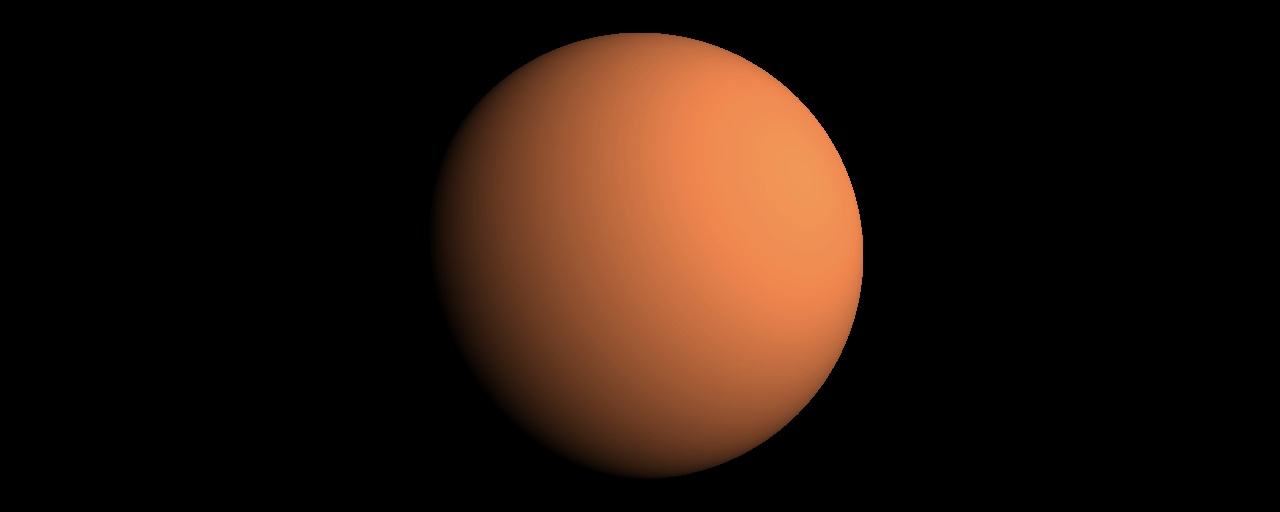
\includegraphics[clip,width=70mm]{ray.png}
  \caption{一}
  \label{fig:sobelx_one}
  \end{center}
  \end{minipage}
  \end{tabular}
  \end{figure}

これは,レイトレーシング(Geforce RTXのアレ)です.これもプログラミング言語を用いて作成することができます.実際にこれはぼくが書いたプログラムによって作成された代物です.
レイトレーシングにおいては,数学の知識をかなり使うのでなかなかやりがいがあると思います.また,processingというpythonに似た優しい言語を使うので,やりやすいと思います.

\url{https://www.raytracing.xyz/}

(対象ユーザーが小学生以上とかいう煽り)

\hrulefill

さらに発展させて,数学とプログラミングを合わせる方向で行くなら競技プログラミングをお勧めします.

\url{https://atcoder.jp/}

これやると数学力が相当つく代わりに計算力が落ちるそうです.しかし,頑張れば基本的になんとかなります.

\subsection{2について}
2はなんらかの目標があって,それを実現するためにしぶしぶ必要になって(手動でやるのがバカバカしすぎるために)やるものばっかりです.例えば,youtube等の動画サイトから動画を(違法に)落としてくるツールの作成(youtube-dl)や,点字ブロックを画像から検出するツール,月と地球の軌道を計算するツール等々.程よく簡単な目標として(休校期間中だらけないようにぼくがやっているもの),"日本語は横書きも縦書きも可能だが,英語は横書き限定である.これは日本語と英語その他の言語における文字について,縦線と横線の割合は異なることによるものか."という目標があるとして,各言語の縦線と横線の割合を自動で計算するプログラムの作成.とかがあります.(身近にある疑問を解決する時にこの力技を使うとすごく楽しいです.)

\begin{itemize}
  \item 0からつくるdeeplearning:有名です. \url{https://www.amazon.co.jp/dp/4873117585}
\end{itemize}

\subsection{3について}
これは完全に変態向けです.いわゆるコンパイラやOSなどを作る爆絶変態コースです.
完成させると,相当の技術力がつきますが,途中まで進めてもかなりの知識がつくと思います.
わたしの先輩にはブラウザを作ったバケモノがいます.


\begin{itemize}
  \item コンパイラの作り方: \url{https://www.sigbus.info/compilerbook}
  \item ブラウザの作り方: \url{https://limpet.net/mbrubeck/2014/08/08/toy-layout-engine-1.html}
  \item osの作り方: \url{https://www.amazon.co.jp/dp/4839919844}
  \item cpuのエミュレーターの作り方:は? \url{https://book.rvemu.app/}
\end{itemize}



\subsection{おまけ}
\begin{itemize}
  \item 群衆の叡智:Twitterを使うものとしては履修しておきたいよね.

  \url{https://ncase.me/crowds/ja.html}

  \item 東大の講習会:これが無料ってまじ?

  \url{http://ong.iis.u-tokyo.ac.jp/ong-steam-stream/}

  \item 東大のスパコン講習:読むと計算機がどうやって動いているかわかるかも.

  \url{https://www.cc.u-tokyo.ac.jp/events/lectures/materials/}

  \item スパコンプログラマ入門:一週間でなれるらしいぜ.

  \url{https://github.com/qulacs/quantum-native-dojo}

  \item 量子コンピュータ入門:すげえ,重ね合わせエンジニアだ.

  \url{https://github.com/qulacs/quantum-native-dojo}

  \item 漢字の成り立ちについて:全然かんけえねえけど.

  \url{https://note.com/nkay/n/n749b4ac54acb}

  \item やりきる能力について:ぼくは途中で捨てがちです.

  \url{https://www.nature.com/articles/s42003-020-0930-4.pdf}
\end{itemize}




\end{document}
